\section{从一条指令到一次推理}
\label{sec:01-system-overview-01}

本节要回答的核心问题是：一段程序究竟是怎样一步步变成硬件上的动作的？
理解这条链路，是后面每一章能够“接着往下搭”的前提。硬件与软件的分工
可参考经典教材\citep{patterson2020}。

本节与后续各章共用同一条主线：同一条指令、同一颗处理器核、同一块开发板，
每一章只在这个系统上增加一层能力。

\begin{figure}[htbp]
\centering
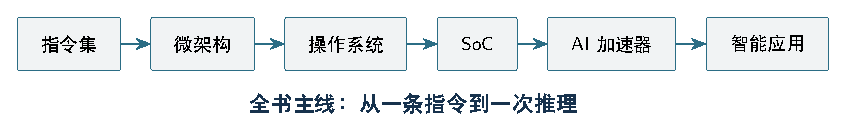
\includegraphics[width=.96\linewidth]{figures/system-stack}
\caption{全书主线：从一条指令到一次推理}
\label{fig:system-stack}
\end{figure}

\begin{definition}[指令集架构]
指令集架构（ISA）是软件与硬件之间的契约，规定了可见的寄存器、指令语义、
数据类型与异常行为；它不规定这些行为由怎样的电路实现。
\end{definition}

% TODO：撰写本节正文。建议结构：
%   1) 问题引入与学习目标
%   2) 原理与机制（配图、公式）
%   3) 示例或实验步骤
%   4) 小结与思考题
本节待撰写。为便于分工，正文请按“概念—机制—示例”的顺序展开，
并在每小节末尾留出一段可以动手验证的实验说明。
